\begin{figure}
\centering
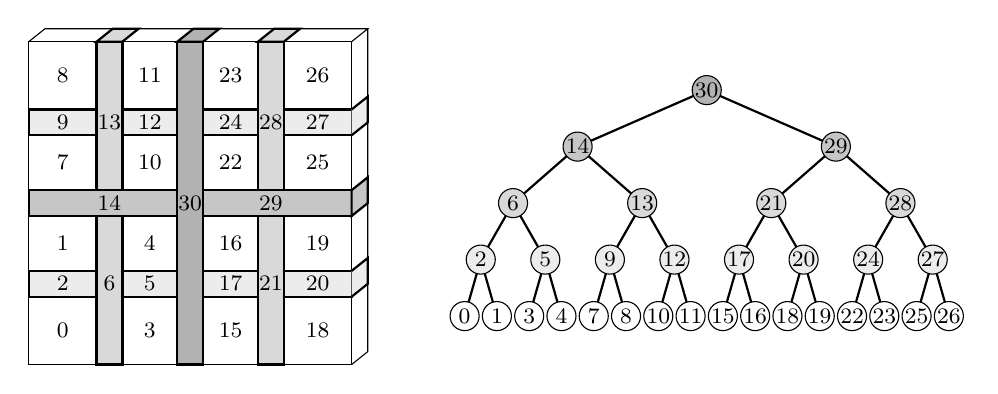
\begin{tikzpicture}[scale=4.1]
\tikzstyle{every node}=[font=\footnotesize]

% Main box
\draw (0,0) rectangle (1,1);
\draw (0,1) -- (0.05,1.04) -- (1.05,1.04) -- (1,1);
\draw (1,0) -- (1.05,0.04) -- (1.05,1.04);

% Root separator
\draw[thick,fill=gray!60!] (0.46,0) rectangle (0.54,1); 
\draw (0.5,0.5) node{$30$};
\draw[thick,fill=gray!60!] 
  (0.46,1) -- (0.51,1.04) -- (0.59,1.04) -- (0.54,1) -- cycle;

% Second level left separator
\draw[thick,fill=gray!45!] (0,0.46) rectangle (0.46,0.54); 
\draw (0.25,0.5) node {$14$};
% Second level right separator
\draw[thick,fill=gray!45!] (0.54,0.46) rectangle (1,0.54); 
\draw (0.75,0.5) node {$29$};
\draw[thick,fill=gray!45!]
  (1,0.54) -- (1.05,0.58) -- (1.05,0.50) -- (1,0.46) -- cycle;

% Third level bottom-left separator
\draw[thick,fill=gray!30!] (0.21,0) rectangle (0.29,0.46); 
\draw (0.25,0.25) node {$6$};
% Third level bottom-right separator
\draw[thick,fill=gray!30!] (0.71,0) rectangle (0.79,0.46); 
\draw (0.75,0.25) node {$21$};
% Third level top-left separator
\draw[thick,fill=gray!30!] (0.21,0.54) rectangle (0.29,1); 
\draw (0.25,0.75) node {$13$};
\draw[thick,fill=gray!30!] 
  (0.21,1) -- (0.26,1.04) -- (0.34,1.04) -- (0.29,1) -- cycle;
% Third level top-right separator
\draw[thick,fill=gray!30!] (0.71,0.54) rectangle (0.79,1); 
\draw (0.75,0.75) node {$28$};
\draw[thick,fill=gray!30!]
  (0.71,1) -- (0.76,1.04) -- (0.84,1.04) -- (0.79,1) -- cycle;

% Fourth level, bottom-left, left
\draw[thick,fill=gray!15!] (0,0.21) rectangle (0.21,0.29); 
\draw (0.105,0.25) node {$2$};
% Fourth level, bottom-left, right
\draw[thick,fill=gray!15!] (0.29,0.21) rectangle (0.46,0.29); 
\draw (0.375,0.25) node {$5$};
% Fourth level, top-left, left
\draw[thick,fill=gray!15!] (0,0.71) rectangle (0.21,0.79); 
\draw (0.105,0.75) node {$9$};
% Fourth level, top-left, right
\draw[thick,fill=gray!15!] (0.29,0.71) rectangle (0.46,0.79); 
\draw (0.375,0.75) node {$12$};
% Fourth level, bottom-right, left
\draw[thick,fill=gray!15!] (0.54,0.21) rectangle (0.71,0.29); 
\draw (0.625,0.25) node {$17$};
% Fourth level, bottom-right, right
\draw[thick,fill=gray!15!] (0.79,0.21) rectangle (1,0.29); 
\draw (0.895,0.25) node {$20$};
\draw[thick,fill=gray!15!]
  (1,0.29) -- (1.05,0.33) -- (1.05,0.25) -- (1,0.21);
% Fourth level, top-right, left
\draw[thick,fill=gray!15!] (0.54,0.71) rectangle (0.71,0.79); 
\draw (0.625,0.75) node {$24$};
% Fourth level, top-right, right
\draw[thick,fill=gray!15!] (0.79,0.71) rectangle (1,0.79); 
\draw (0.895,0.75) node {$27$};
\draw[thick,fill=gray!15!]
  (1,0.79) -- (1.05,0.83) -- (1.05,0.75) -- (1,0.71);

\draw (0.105,0.105) node {$0$};
\draw (0.105,0.375) node {$1$};
\draw (0.375,0.105) node {$3$};
\draw (0.375,0.375) node {$4$};

\draw (0.105,0.625) node {$7$};
\draw (0.105,0.895) node {$8$};
\draw (0.375,0.625) node {$10$};
\draw (0.375,0.895) node {$11$};

\draw (0.625,0.105) node {$15$};
\draw (0.625,0.375) node {$16$};
\draw (0.895,0.105) node {$18$};
\draw (0.895,0.375) node {$19$};

\draw (0.625,0.625) node {$22$};
\draw (0.625,0.895) node {$23$};
\draw (0.895,0.625) node {$25$};
\draw (0.895,0.895) node {$26$};

%\draw (1.3,0) rectangle (2.9,1);

% Draw the connections between the bottom and second level nodes
\draw[thick] (1.35,0.15) -- (1.4,0.325) -- (1.45,0.15);
\draw[thick] (1.55,0.15) -- (1.6,0.325) -- (1.65,0.15);
\draw[thick] (1.75,0.15) -- (1.8,0.325) -- (1.85,0.15);
\draw[thick] (1.95,0.15) -- (2.0,0.325) -- (2.05,0.15);
\draw[thick] (2.15,0.15) -- (2.2,0.325) -- (2.25,0.15);
\draw[thick] (2.35,0.15) -- (2.4,0.325) -- (2.45,0.15);
\draw[thick] (2.55,0.15) -- (2.6,0.325) -- (2.65,0.15);
\draw[thick] (2.75,0.15) -- (2.8,0.325) -- (2.85,0.15);

% Draw the connections between the second and third level nodes
\draw[thick] (1.4,0.325) -- (1.5,0.500) -- (1.6,0.325);
\draw[thick] (1.8,0.325) -- (1.9,0.500) -- (2.0,0.325);
\draw[thick] (2.2,0.325) -- (2.3,0.500) -- (2.4,0.325);
\draw[thick] (2.6,0.325) -- (2.7,0.500) -- (2.8,0.325);

% Draw the connections between the third and fourth level nodes
\draw[thick] (1.5,0.500) -- (1.7,0.675) -- (1.9,0.500);
\draw[thick] (2.3,0.500) -- (2.5,0.675) -- (2.7,0.500);

% Draw the connections to the root note
\draw[thick] (1.7,0.675) -- (2.1,0.85) -- (2.5,0.675);

% Draw the bottom nodes
\draw[fill=white] (1.35,0.15) circle (0.045); \draw (1.35,0.15) node{$0$};
\draw[fill=white] (1.45,0.15) circle (0.045); \draw (1.45,0.15) node{$1$};
\draw[fill=white] (1.55,0.15) circle (0.045); \draw (1.55,0.15) node{$3$};
\draw[fill=white] (1.65,0.15) circle (0.045); \draw (1.65,0.15) node{$4$};
\draw[fill=white] (1.75,0.15) circle (0.045); \draw (1.75,0.15) node{$7$};
\draw[fill=white] (1.85,0.15) circle (0.045); \draw (1.85,0.15) node{$8$};
\draw[fill=white] (1.95,0.15) circle (0.045); \draw (1.95,0.15) node{$10$};
\draw[fill=white] (2.05,0.15) circle (0.045); \draw (2.05,0.15) node{$11$};
\draw[fill=white] (2.15,0.15) circle (0.045); \draw (2.15,0.15) node{$15$};
\draw[fill=white] (2.25,0.15) circle (0.045); \draw (2.25,0.15) node{$16$};
\draw[fill=white] (2.35,0.15) circle (0.045); \draw (2.35,0.15) node{$18$};
\draw[fill=white] (2.45,0.15) circle (0.045); \draw (2.45,0.15) node{$19$};
\draw[fill=white] (2.55,0.15) circle (0.045); \draw (2.55,0.15) node{$22$};
\draw[fill=white] (2.65,0.15) circle (0.045); \draw (2.65,0.15) node{$23$};
\draw[fill=white] (2.75,0.15) circle (0.045); \draw (2.75,0.15) node{$25$};
\draw[fill=white] (2.85,0.15) circle (0.045); \draw (2.85,0.15) node{$26$};

% Draw the second level of nodes
\draw[fill=gray!15!] (1.4,0.325) circle (0.045); \draw (1.4,0.325) node{$2$};
\draw[fill=gray!15!] (1.6,0.325) circle (0.045); \draw (1.6,0.325) node{$5$};
\draw[fill=gray!15!] (1.8,0.325) circle (0.045); \draw (1.8,0.325) node{$9$};
\draw[fill=gray!15!] (2.0,0.325) circle (0.045); \draw (2.0,0.325) node{$12$};
\draw[fill=gray!15!] (2.2,0.325) circle (0.045); \draw (2.2,0.325) node{$17$};
\draw[fill=gray!15!] (2.4,0.325) circle (0.045); \draw (2.4,0.325) node{$20$};
\draw[fill=gray!15!] (2.6,0.325) circle (0.045); \draw (2.6,0.325) node{$24$};
\draw[fill=gray!15!] (2.8,0.325) circle (0.045); \draw (2.8,0.325) node{$27$};

% Draw the third level of nodes
\draw[fill=gray!30!] (1.5,0.500) circle (0.045); \draw (1.5,0.500) node {$6$};
\draw[fill=gray!30!] (1.9,0.500) circle (0.045); \draw (1.9,0.500) node {$13$};
\draw[fill=gray!30!] (2.3,0.500) circle (0.045); \draw (2.3,0.500) node {$21$};
\draw[fill=gray!30!] (2.7,0.500) circle (0.045); \draw (2.7,0.500) node {$28$};

% Draw the fourth level of nodes
\draw[fill=gray!45!] (1.7,0.675) circle (0.045); \draw (1.7,0.675) node {$14$};
\draw[fill=gray!45!] (2.5,0.675) circle (0.045); \draw (2.5,0.675) node {$29$};

% Draw the root node
\draw[fill=gray!60!] (2.1,0.85) circle (0.045); \draw (2.1,0.85) node {$30$};

\end{tikzpicture}
\caption{A separator-based supernodal elimination tree (right) over a 
  quasi-2D subdomain (left).}
\label{fig:sep-tree}
\end{figure}
